\documentclass[11pt,a4paper,english]{article}
\usepackage[english]{babel} % Using babel for hyphenation
\usepackage{lmodern} % Changing the font
\usepackage[utf8]{inputenc}
\usepackage[T1]{fontenc}

%\usepackage[moderate]{savetrees} % [subtle/moderate/extreme] really compact writing
\usepackage{tcolorbox}
\tcbuselibrary{hooks}
\usepackage[parfill]{parskip} % Removes indents
\usepackage{amsmath} % Environment, symbols etc...
\usepackage{amssymb}
\usepackage{framed}
\usepackage{float} % Fixing figure locations
\usepackage{multirow} % For nice tables
%\usepackage{wasysym} % Astrological symbols
\usepackage{graphicx} % For pictures etc...
\usepackage{enumitem} % Points/lists
\usepackage{physics} % Typesetting of mathematical physics examples: 
                     % \bra{}, \ket{}, expval{}
\usepackage{url}
\usepackage{mathtools}
\usepackage{graphicx}
\usepackage{caption}
\usepackage{subcaption}
\newenvironment{algorithm}{%
\refstepcounter{algcounter}
\begin{tcolorbox}
\centerline{Algorithm \thealgcounter}\vspace{2mm}
}
{\end{tcolorbox}}

\definecolor{red}{RGB}{255,10,10}
\definecolor{pink}{RGB}{255,20,147}

% To include code(-snippets) with æøå
\usepackage{listings}
\lstset{
language=c++,
showspaces=false,
showstringspaces=false,
frame=l,
}

\tolerance = 5000 % Bedre tekst
\hbadness = \tolerance
\pretolerance = 2000

\numberwithin{equation}{section}

\newcommand{\conj}[1]{#1^*}
\newcommand{\ve}[1]{\mathbf{#1}} % Vektorer i bold
\let\oldhat\hat
\renewcommand{\hat}[1]{\oldhat{#1}}
\newcommand{\trans}[1]{#1^\top}
\newcommand{\herm}[1]{#1^\dagger}
%\renewcommand{\thefootnote}{\fnsymbol{footnote}} % Gir fotnote-symboler
\newcommand{\Real}{\mathbb{R}}
\newcommand{\bigO}[1]{\mathcal{O}\left( #1 \right)}

\renewcommand{\thesection}{\Roman{section}} 
\renewcommand{\thesubsection}{\thesection.\Roman{subsection}}

\newcommand{\spac}{\hspace{5mm}}

\newcounter{algcounter}
\newcommand{\algnum}{\stepcounter{algcounter}\Roman{algcounter}}

\title{MEK4300 - Mandatory assignment 1}
\author{Krister Stræte Karlsen}
\date{\today}

\begin{document}
\tcbset{before app=\parfillskip0pt}
\maketitle

\section{Poiseuille flow through ducts}

Poiseuille flow through ducts are goverened by the equation 
\begin{equation}
\nabla^2 u = -\frac{1}{\mu}\left( \frac{dp}{dx} \right)_0  
\end{equation}
with no-slip on the boundaries.  

The numerical solution of three different duct flows have been computed using the finite element method in FEniCS and compared to the analytical solutions (3-47), (3-49) and (3-52) in White.  

Results obtained from experimenting with mesh densities and different order polynomials for the solution are found in Table 1.

\begin{figure}[h!] 
\begin{center}
  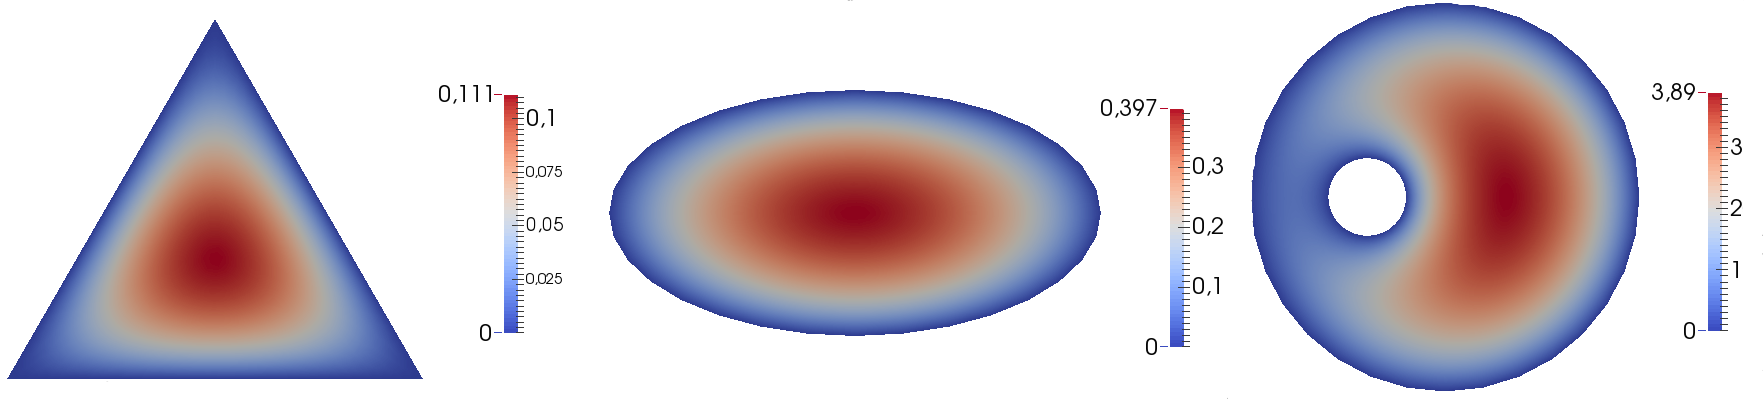
\includegraphics[scale=0.2]{ducts.png}
  \end{center}
  \caption{Numerical solutions obtained using FEniCS corresponding to (3-47), (3-49) and (3-52) in White.}
\end{figure}

For the triangle duct the results are very good and exactly what we would expect from using first and second order polynomials for the solution. 

However, for the ellipse the rate of convergence gets no better than 2 for polynomials of any order(which is what we would expect for linear polynomials). Why is this? The geometry that we approximate by triangles will never have a curved boundary as it should have. The boundary will always consist of piece-wise straight lines(linear), and that is why we cannot get better convergence rate than for linear polynomials.    

\begin{table}[H]
\centering
\caption{Mesh density($h$), error($E$) and convergence rate from comparing the numerical solution(FEniCS) with the analytic solution in White for the velocity(for triangle and ellipse) and flux(eccentric annulus). }
\vspace{3mm}
\begin{tabular}{|l|l|l|l|l|l|l|l|}
\hline
 \multicolumn{6}{|c|}{\textbf{Triangle}}   \\
\hline
 \multicolumn{3}{|c|}{ \textsc{1st order polynomial}} &  \multicolumn{3}{|c|}{\textsc{2nd order polynomial}}  \\
\hline
$h$ & $E$ & $r$ & $h$ & $E$ & $r$   \\
\hline
0.25718 & 0.00240 & 0.34159	& 0.25718 & 9.01820e-05 & 1.05622 \\
0.12859 & 0.00060 & 2.00835	& 0.12859 & 1.21251e-05 & 2.89484 \\
0.06430 & 0.00015 & 2.03221 & 0.06430 & 1.55805e-06 & 2.96018	\\ 
\hline
 \multicolumn{6}{|c|}{\textbf{Ellipse}}   \\
\hline
 \multicolumn{3}{|c|}{ \textsc{1st order polynomial}} &  \multicolumn{3}{|c|}{\textsc{2nd order polynomial}}  \\
\hline
$h$ & $E$ & $r$ & $h$ & $E$ & $r$   \\
\hline
0.12117 & 1.61159e-05 & 1.81054 & 0.05915 & 2.10289e-05 & 1.88642 \\
0.05728 & 3.92276e-06 & 1.88613 & 0.02860 & 5.23161e-06 & 1.91519 \\
0.02940 & 9.72981e-07 & 2.09094 & 0.01398 & 1.29971e-06 & 1.94568 \\
\hline
 \multicolumn{6}{|c|}{\textbf{Eccentric annulus}}   \\
\hline
 \multicolumn{3}{|c|}{ \textsc{1st order polynomial}} &  \multicolumn{3}{|c|}{\textsc{2nd order polynomial}}  \\
\hline
$h$ & $E$ & $r$ & $h$ & $E$ & $r$   \\
\hline
0.28848 & 0.02525 & 9.15876 & 0.28848 & 0.01443 & 0.42121 \\
0.14421 & 0.01724 & 0.55034 & 0.14421 & 0.01428 & 0.01536 \\
0.06849 & 0.01505 & 0.18240 & 0.06849 & 0.01423 & 0.00454 \\
\hline
\end{tabular}
\label{tab:time}
\end{table}

The results we obtain for the eccentric annulus impress nobody. For first order polynomials the error is decreasing as the mesh is refined, but the convergence rates are very low. For second order polynomials it seems that the best obtainable solution is already reached for the coarsest mesh, and the solution does not improve. 

The most likely reason for this is that the author has failed to implement the analytic solution correctly, as it is one !$\star \Box \dagger$ of an expression. Other trivial programming mistakes may, based on experience, also have occurred.



\section{Solving nonlinear equations using FEniCS}

\textbf{Plane stagnation flow}

The equation for plane stagnation flow can be written as
\begin{equation}
F''' + FF' + 1 - (F')^2 = 0
\end{equation}
with $F(0) = F'(0) = 0$ and $F'(\infty)=1$.

This nonlinear equation can be solved as a system of equations using a variational formulation and a mixed function space. We get the following system by letting $H=F'$
\begin{align}
H - F' = 0, \\
H'' + FH' + 1 - H^2 = 0.
\end{align}
We must then find $F,H \in V \cross Q$ such that 
\begin{align*}
\int_\Omega v_h(H - F') dx =0 \quad \forall \quad v_h \in V, \\
\int_\Omega v_f(H'' + FH' + 1 - H^2) dx = 0 \quad \forall \quad  v_f \in Q.
\end{align*}
To obtain a weak formulation we can just integrate the first term in the second equation by parts. 

This equation is easily solved with Newtons method in FEniCS.

\begin{figure}[h!]
\begin{center}
  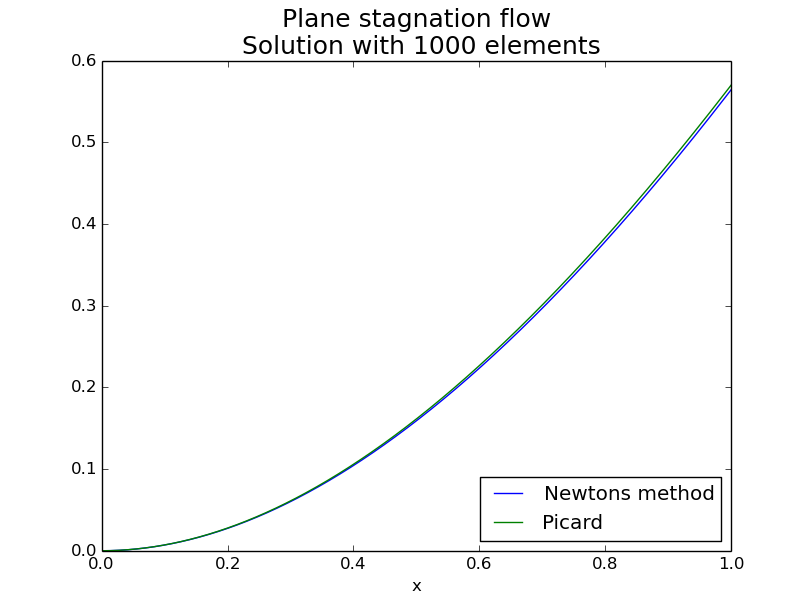
\includegraphics[scale=0.4]{plane_stag.png}
  \end{center}
  \caption{Plot of the equation for plane stagnation flow.}
  \label{fig:stokes_square}
\end{figure}

To solve this equation using Picard iterations in FEniCS we need an initial guess $F_0$ and iterate until the difference, $\epsilon$ between the guess and $F$ becomes sufficiently small. A good guess can be  for instance $x$, as it obeys two of the boundary conditions and looks like the shape of $F$ when $x$ becomes large.   

In Figure 2 we can see that both Newtons method and Picard give very similar solutions that obey the boundary conditions. The slope of the solution rapidly approaches $1$ as we would expect it too.     
\newpage
\textbf{Axisymmetric stagnation flow}

The equation for axisymmetric stagnation flow can be written as
\begin{equation}
F''' + 2FF' + 1 - (F')^2 = 0
\end{equation}
with $F(0) = F'(0) = 0$ and $F'(\infty)=1$.

\begin{figure}[h!]
\begin{center}
  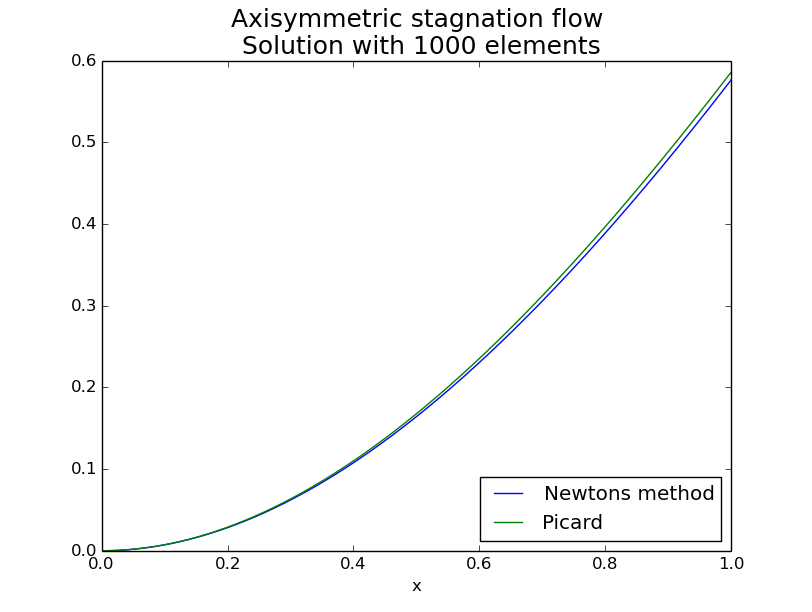
\includegraphics[scale=0.4]{axisym_stag.png}
  \end{center}
  \caption{Plot of the equation for axisymmetric stagnation flow}
  \label{fig:stokes_square}
\end{figure}

We solve this equation in similar manner and the solution we obtain is of the same shape as for plane stagnation flow, see Figure 3. That comes as no surprise as the equation only differs by a factor of 2 in one of the terms.   

\section{Stokes flow for a driven cavity}
Flows at very low Reynolds numbers are often called \emph{Stokes flow} and are governed by the equations 
\begin{equation}
\mu \nabla^2 \mathbf{u} = \nabla p
\end{equation}
\begin{equation}
\nabla \cdot \mathbf{u} = 0.
\end{equation}

We will have a look at Stokes flow for a driven cavity in the domain $\Omega = [0,1] \cross [0,1]$ where the top wall i moving with velocity $\mathbf{u} = (1,0)$ and the remaining three walls are at rest. For a graphical interpretation of the problem see Figure \ref{fig:stokes_square}. FEniCS well be used to compute the solution. 

\begin{figure}[h!]
\begin{center}
  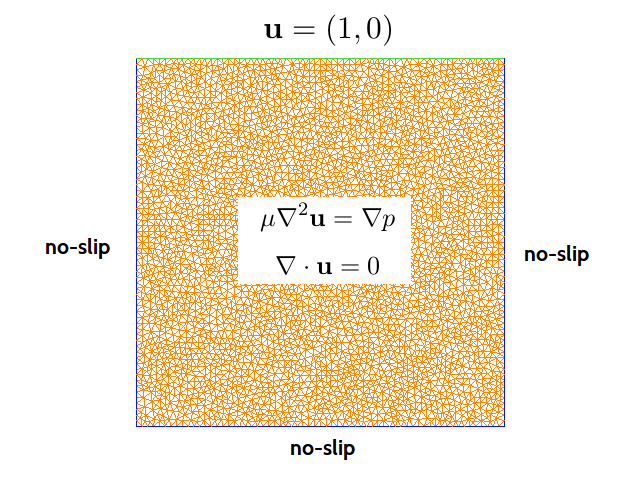
\includegraphics[scale=0.3]{stokes_square.png}
  \end{center}
  \caption{Illustration of the problem(iii) and the domain.}
  \label{fig:stokes_square}
\end{figure}

To solve this problem using FEniCS we need the variational formulation, which for this problem is
\begin{equation}
\mu \int_\Omega \nabla \mathbf{v}:\nabla \mathbf{u} dx = \int_\Omega p \nabla \cdot \mathbf{v} dx 
\end{equation}
\begin{equation}
\mu \int_\Omega p\nabla \cdot \mathbf{u} dx = 0.
\end{equation}

This variational formulation involves both a scalar test function $q$, and a vector test function $\mathbf{v}$. We will solve this as a coupled problem using \emph{Taylor-Hood elements}; A an triangular element commonly used for Stokes flow where the velocity is approximated by a polynomial of higher degree than the pressure. 

\begin{figure}[h!]
\begin{center}
  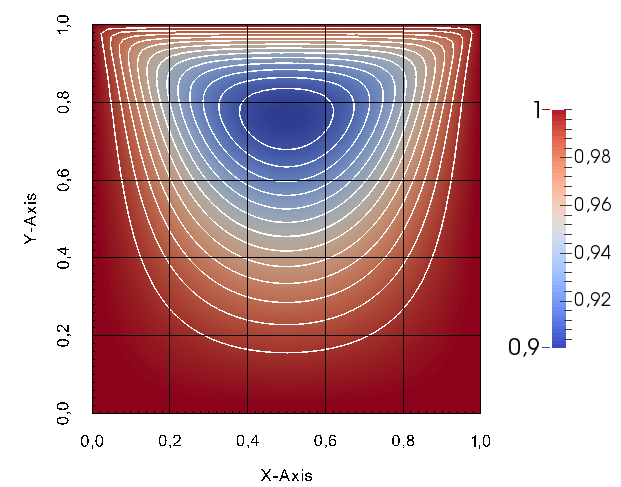
\includegraphics[scale=0.4]{psi_square.png}
  \end{center}
  \caption{Plot of the stream function with contour lines for driven cavity flow.}
\end{figure}

We want to see if we can locate the center of a vortex in the cavity flow by computing the stream function $\psi$ , and see where it goes through a minimum. The stream function can be computed in similar manner, by using a variational formulation,  
\begin{equation}
-\int_\Omega \nabla \phi \cdot \nabla \psi dx + \int_{\partial \Omega} \phi \nabla \psi \cdot \mathbf{n} ds = - \int_\Omega \phi \omega dx.
\end{equation}

However, in this case the integral over the boundary is dropped as the boundary conditions are Dirichlet.
A contour plot of the stream function is featured in Figure 3 and the exact location of the vortex was computed to be 

\texttt{[x,y] =  [0.50133195 , 0.76516977].}

The results obtained by minimizing the stream function seems to be in agreement with the "by-the-eye-approach" of looking at Figure 5.  


\section{Stokes flow past a step}

We will here look at a model for Stokes flow past a step with a moving top plate. See figure 6.

\begin{figure}[h!]
\begin{center}
  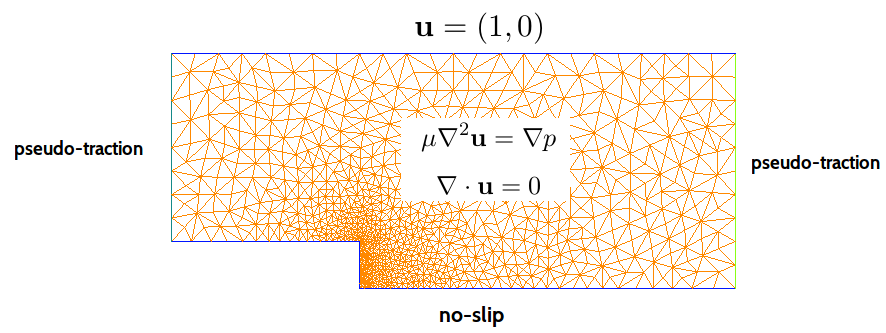
\includegraphics[scale=0.3]{stokes_step.png}
  \end{center}
  \caption{Illustration of the problem(iv) and the domain.}
\end{figure}

Now, with an inlet and an outlet in our domain, we need some boundary conditions allowing fluid to flow through the boundaries. A good choice is something called a \emph{pseudo-traction boundary condition}. It is really nothing but a trick to let fluid enter and exit the domain with little interference of the boundary, and it is implemented my simply doing nothing. 

Another choice of boundary condition could be a linear velocity profile at the entrance and fixed pressure at the exit. Such conditions would make sense if the distance between the entrance and the step was big and the exit were really an exit into another fluid where the pressure was known. 

I implemented both and noticed little or no difference. 
\newpage
\textbf{(a) Vortex}

The vortex location is hunted down in similar manner this time. The only difference now is that we must include a boundary term in the variational form since we have no Dirichlet conditions to enforce.

The obtained location as a function of mesh density is presented in Table 2.

\begin{table}[H]
\centering
\caption{ Mesh density(\texttt{mesh.hmin()}) and vortex location. }
\vspace{3mm}
\begin{tabular}{|l|l|l|l|l|}
\hline
\textbf{Mesh density} & \textbf{Vortex location}    \\
\hline
0.009893 & [0.43550429 , 0.03588525]   \\
\hline
0.004946 & [0.43455854 , 0.03908434]	   \\
\hline
0.002473 & [0.43455854 , 0.03908434]    \\ 
\hline
\end{tabular}
\label{tab:time}
\end{table}

The computed location of the vortex rapidly approaches $[x,y] \simeq [0.43, 0.04]$ as the mesh is refined. These results are in agreement with the graphics produced in ParaView. See Figure 7. 


\textbf{(b) The stream function}

The stream function was computed and a contour plot made using ParaView. Only the lowest value contours were kept to make the data of interest easily observable. See figure 7. 

\begin{figure}[h!]
\begin{center}
  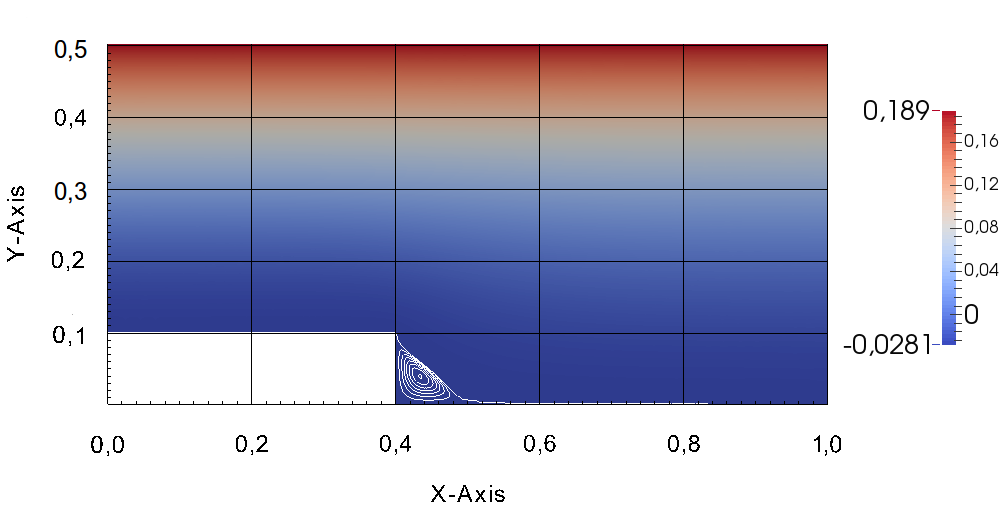
\includegraphics[scale=0.30]{psi_step.png}
  \end{center}
  \caption{Contours in lowest range of values for the stream function.}
\end{figure}

\textbf{(c) Flux and conservation of mass}

The flux, given by 
\begin{align*}
Q = \int_{\Gamma} u dA,
\end{align*}
is computed in FEniCS over the inlet and the outlet to be:

\noindent
\texttt{Inlet flux:  -0.216791938563} \\
\texttt{Outlet flux:  0.216791938563} \\
\texttt{Difference in influx/outflux: -1.16573417586e-15}

Mass seems to be conserved. 


\textbf{(d) Reversed direction of flow}

Reversing the direction of the flow we find the same location for the vortex:

\texttt{Location of vortex(reversed) [x,y]:  [0.43455854 , 0.03908434] }

Why this is, becomes very clear by looking at the equation for the stream function. Here assuming a 2D case.
\begin{align*}
\nabla \psi = \partial_x \psi + \partial_y = -v \mathbf{i} + u \mathbf{j} \\
\nabla \cdot \nabla \psi = \nabla^2 \psi = -\partial_x v + \partial_y u = -\omega 
\end{align*} 
Now, taking the curl of equation (III.1) we find that $\nabla^2 \omega= 0$. Inserting this into the last equation above we obtain a \emph{biharmonic equation} for $\psi$, 
\begin{align*}
\nabla^4 \psi = 0.
\end{align*} 
It is now easy to understand that if $\psi$ is a solution, then $-\psi$ must be a solution as well. Only the flow direction in the vortex is changed, see Figure  8-9 on the last page.  



\textbf{(e) Normal stress on wall} \\

The stress in a viscous fluid is given by 
\begin{equation}
\tau = -pI + \mu (\nabla \mathbf{u}  + \nabla \mathbf{u}^T  ) = pressure + \textit{shear stress}. 
\end{equation}

The shear stress does not contribute to normal stress so we get get this simple expression for the normal stress
\begin{align*}
\int_{S} (-p I \cdot \mathbf{n} ) \cdot \mathbf{n} \quad ds.
\end{align*}

The results we get from computing the normal stress for both directions are:

\texttt{Normal stress:  132.813411229} \\
\texttt{Normal stress(reversed):  -132.813411229 }

Only the sign differs for the different flow directions. 
\newpage


\begin{figure*}[t!]
    \centering
    \begin{subfigure}[b]{0.5\textwidth}
        \centering
        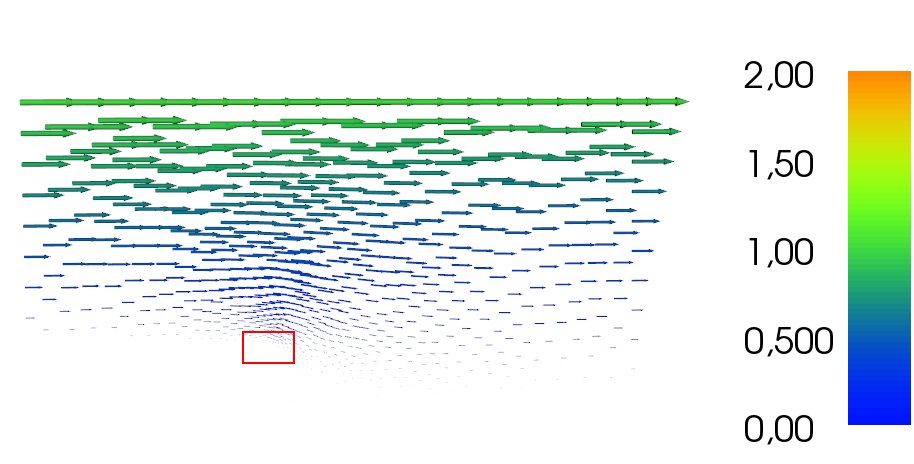
\includegraphics[scale=0.25]{vel_step1.png}
        \caption{Full velocity field.}
    \end{subfigure}%
    ~ 
    \begin{subfigure}[b]{0.5\textwidth} 
        \centering
        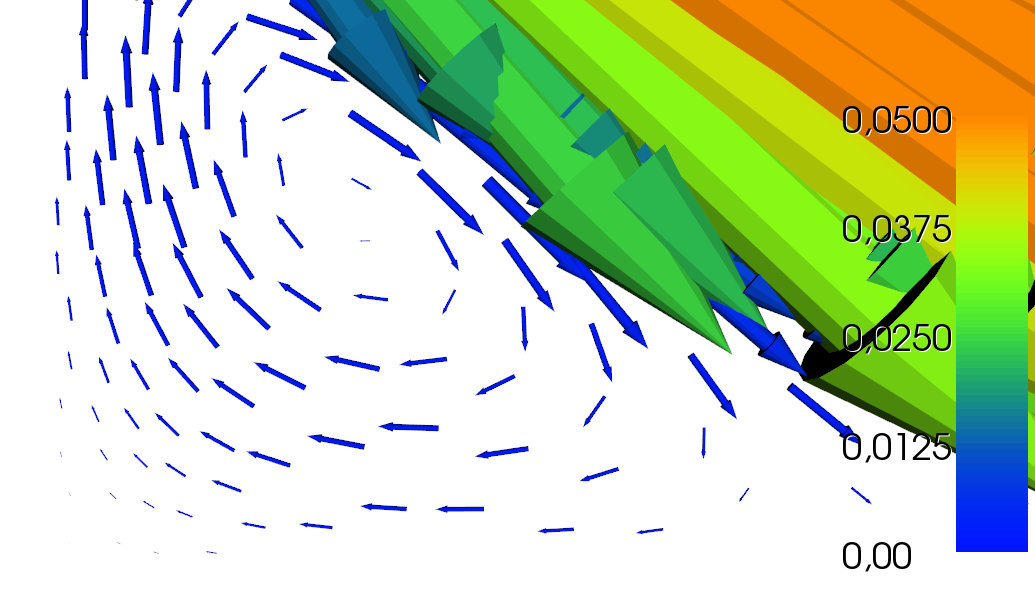
\includegraphics[scale=0.18]{vel_step2.png}
        \caption{Zoomed in a vortex can be observed.}
    \end{subfigure}
    \caption{Velocity field of Stokes flow past a step computed using FEniCS.}
\end{figure*}


\vspace{1.5cm}
\begin{figure}[h!]
\begin{center}
  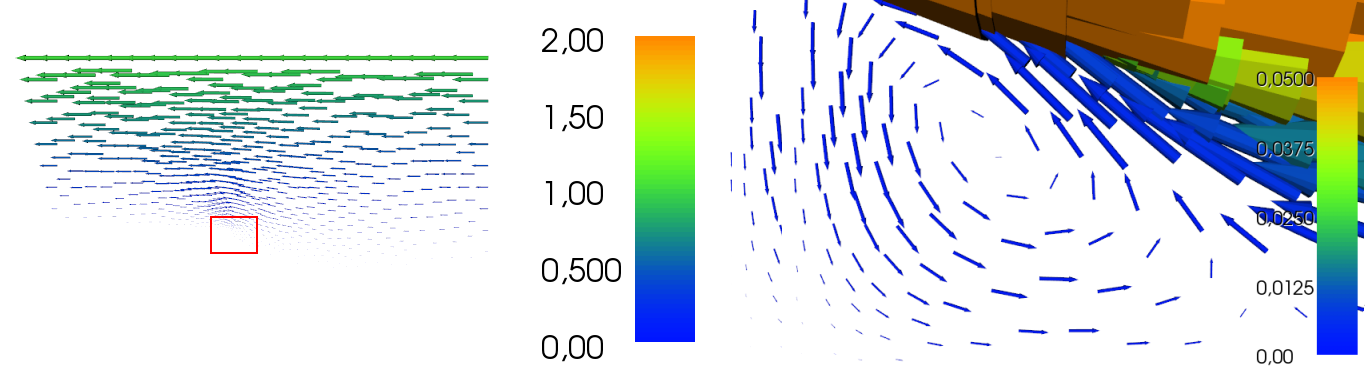
\includegraphics[scale=0.28]{reverse_velstep.png}
  \end{center}
  \caption{Velocity field for flow in the opposite direction.}
\end{figure}



\end{document}
